\chapter{相关工作 }\label{chap:related_work}
% 2.1边缘计算技术,多终端,协同,服务
%     2.2docker容器技术/容器集群技术
%     2.3自组织网络技术——对应研究点1
%     2.4启发式调度算法——对应研究点2  可能会换成任务调度算法
%     2.5计算迁移——对应研究点3
%     2.6预测算法——对应研究点4
\section{云计算技术}
\section{边缘计算技术}


\section{虚拟化技术}
资源管理问题是协同服务技术中的一个重要的问题\citep{文雨2013面向应用服务级目标的虚拟化资源管理}。虚拟化技术是一种资源管理技术,利用底层虚拟、上层隔离等方法,将计算机中的物理资源,如计算、存储和网络等,进行抽象、切割,以更好的形式提供给用户使用[?]。虚拟化技术将计算机上原有的固定配额的物理资源按照用户需要很方便地进行分配、提取和利用,可以提高计算机和终端资源的利用率。1959年,克里斯托弗(Christopher Strachey)在他的学术报告《大型高速计算机中的时间共享》中提出了虚拟化的基本概念,成为了虚拟化技术的开端\citep{本刊编辑部2017虚拟化概述}。在IBM公司、HP公司、VMWare公司等企业的不断努力下,经过了60年的发展和成熟,虚拟化技术逐渐成为云计算与边缘计算中非常重要的一种资源管理技术\citep{pearce2013virtualization}。用户根据自己的需求来租赁云计算或边缘计算的服务提供商所提供的对应资源配额的虚拟机,直接在虚拟化的操作系统中运行用户自己的应用而不需要考虑操作系统底层是如何实现的,就如同运行在一个真实而独立的实体物理机一样,非常透明。而虚拟化技术则被用来实现虚拟机的生命周期管理,包括创建、配置、关闭、监控、释放资源等等,维持这种对用户的透明性。应用了虚拟化技术的云计算模型如图\ref{fig:cloud_computation_virtualization}所示\citep{陈思锦2015云计算中的虚拟化技术与虚拟化安全}。
\begin{figure}[!htbp]
    \centering
    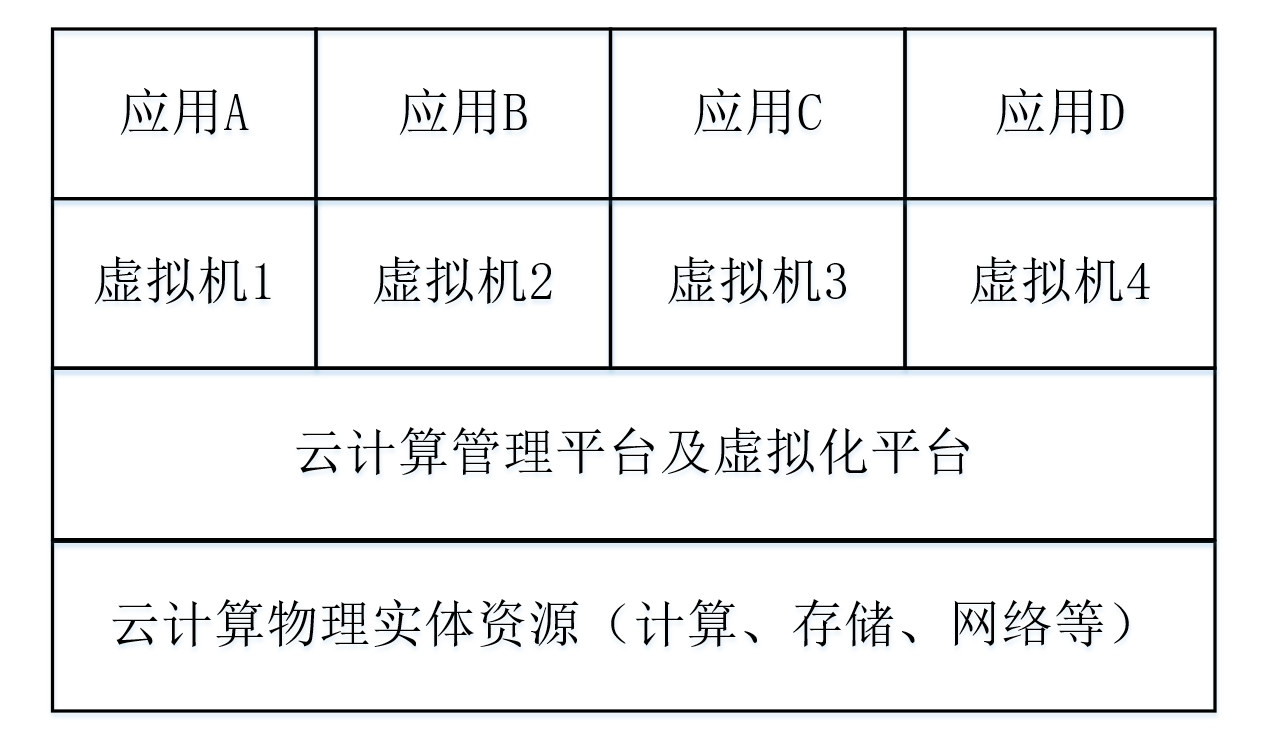
\includegraphics[width=1.0\textwidth]{Cloud_Computation_Virtualization_Temp}
    \caption{应用了虚拟化技术的云计算模型}
    \label{fig:cloud_computation_virtualization}
\end{figure}

\subsection{完全虚拟化技术}

完全虚拟化技术(Full Virtualization Technology)通过在宿主机操作系统(Host Operation System,简称为Host OS)上面架设一层虚拟机监控器(Virtual Machine Monitor,简称为VMM)\citep{li2017performance}来实现对硬件的虚拟化,完全虚拟化技术中的虚拟机监控器,通常为超级监控器,即Hypervisor或者Supervisor\citep{kolhe2012comparative}\citep{leite2012performance}。VMM在虚拟硬件的基础上再进一步虚拟出一套用户的操作系统(Guest Operation System,简称为Guest OS),供用户操作使用。为了方便阐述,在本文中,通过完全虚拟化技术实现的虚拟机简称为VM虚拟机。完全虚拟化技术的架构如图\ref{fig:full_virtualization}所示\citep{oludele2014evolution}。

\begin{figure}[!htbp]
    \centering
    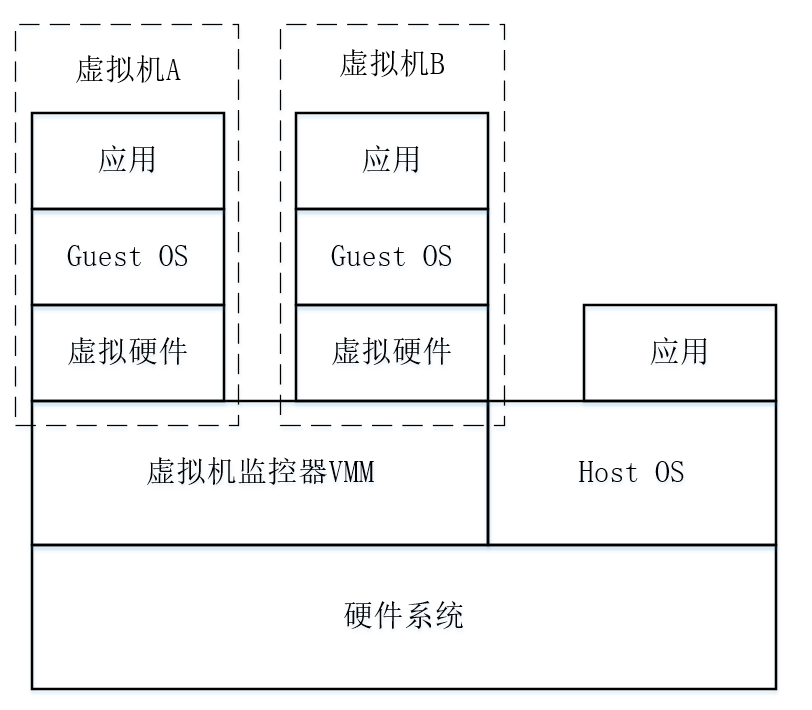
\includegraphics[width=1.0\textwidth]{Full_Virtualization_Temp}
    \caption{完全虚拟化技术架构}
    \label{fig:full_virtualization}
\end{figure}

云计算行业内曾经非常流行的工具如VMware\citep{sahasrabudhe2014comparing}\cite{li2010selecting}、KVM\citep{liu2014research}、VirtualBox\citep{li2010selecting}等,都属于比较传统的完全虚拟化技术,这些完全虚拟化工具都拥有非常良好的对硬件资源的管理、隔离、虚拟、利用的功能。但是另一方面,完全虚拟化技术使用了虚拟机监控器VMM来虚拟硬件层,能够提供相对较完整独立、隔离性好的虚拟化环境,但是启动速度慢,需要消耗大量额外资源来维持虚拟化环境。

\subsection{操作系统级虚拟化技术}

操作系统级虚拟化技术(Operation System Virtualization Technology),是一种轻量级虚拟化技术\citep{morabito2017virtualization}。与传统的完全虚拟化技术相比,操作系统级虚拟化技术不需要对底层硬件进行虚拟化,而是直接在操作系统层上采用隔离的方法虚拟出与宿主机操作系统互相隔离的虚拟机。对此有一个生动形象的比喻,如果将物理实体宿主机比作一座房子,那么其底层硬件则是地基,操作系统是房子的支撑墙,系统中运行的应用则是房子内的具体房间。而传统的完全虚拟化技术可以比喻为在原有房子的地基之上另外实现一层新的地基(虚拟机监控器VMM),并在新地基上重新修建支撑墙(Guest OS)和房间(虚拟机)。相应地,操作系统级虚拟化技术则是直接借用了宿主机原有的地基(底层硬件)和支撑墙(操作系统),并在原来的房间里利用隔板隔离出来新的房间(虚拟机)。操作系统级虚拟化技术的架构如图\ref{fig:os_virtualization}所示\citep{xavier2013performance}。由于没有使用虚拟机监控器VMM来对硬件进行虚拟化,所以操作系统级虚拟化技术启动速度非常快,而且也不会消耗非常多的额外虚拟化开销,非常轻量级\citep{babu2014system}。

\begin{figure}[!htbp]
    \centering
    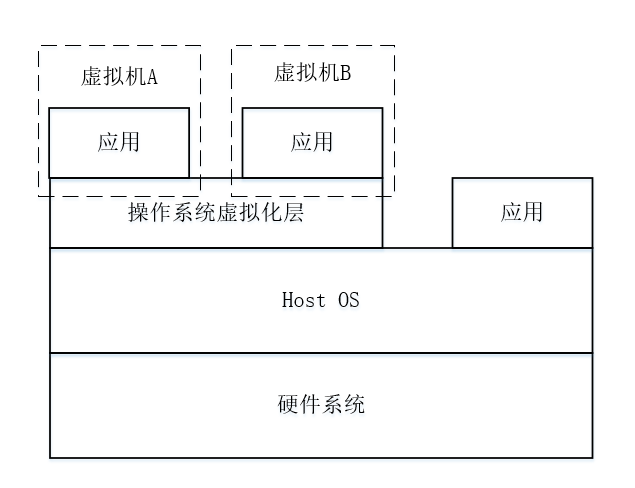
\includegraphics[width=1.0\textwidth]{OS_Virtualization_Temp}
    \caption{操作系统级虚拟化技术架构}
    \label{fig:os_virtualization}
\end{figure}

\subsection{容器虚拟化技术}

容器虚拟化技术(Container Virtualization Technology)属于操作系统级虚拟化技术的一种\citep{vaughan2006new}。容器虚拟化技术虚拟出来的“虚拟机”通常被称为容器(Container)。容器技术底层使用的是基于Linux内核的Linux Container(LXC)技术,而不需要进行额外的虚拟化操作。LXC技术的核心技术包括Namespace技术和Cgroups技术。Namespace技术可以为容器提供一个独立的、隔离的命名空间,其中包含PID(进程)、UTS(host name)、MNT(文件)、NET(网络)、IPC(进程间交互)、USER(用户)等六个方面。不同命名空间的进程彼此之间看不到,Namespace单独隔离出来的命名空间中的容器与其宿主机之间也是彼此看不到,只能通过UTS将对方当作网络中的另一个主机节点,这样就保持了容器的独立性和隔离性。而通过Cgroups技术,可以对每个容器所拥有的CPU、内存、存储、输入输出等资源进行进程级别的管理和配置,这样就使得用户可以利用容器对终端资源进行按需分配管理。同时,利用Cgroups控制组,也能够对对容器内各种资源的消耗情况做监控。因为容器底层仍然是利用宿主机的操作系统,所以相比完全虚拟化技术,容器虚拟化技术基本没有太大的额外性能损耗,启动一个容器也相当于启动一个进程,启动时间基本为秒级时间。目前行业内最流行的基于容器虚拟化技术的产品是Docker\citep{liu2014researchandimplementation}\cite{bernstein2014containers}\cite{马晓光2017一种适用于}。本文中所涉及到的容器虚拟化技术均是使用Docker应用实现的。

% \subsection{容器集群技术}


% \section{自组织网络技术}
\section{计算迁移技术}
\subsection{云计算中的计算迁移技术}
传统的终端设备的服务模式通常是终端设备在本地进行计算任务的运行,依靠终端设备自身的计算能力来保证服务质量。而随着边缘智能终端设备所要承担的计算任务越来越重,单一终端设备本地计算难以满足终端服务和任务对终端计算能力的要求,计算迁移技术逐渐成为了一个可行的解决方案。计算迁移技术,也被称为计算卸载技术(computation offloading),是指将终端设备上的计算任务,通过网络的形式发送到其他设备上进行计算,再将计算结果通过网络返回给终端设备。

在边缘计算中,通常使用的方法是将边缘终端设备上的计算任务根据具体需求迁移一部分或迁移全部到云端计算资源上进行处理。云端计算资源通常是部署在云数据中心的机房,可以提供计算、存储、网络等资源。这种计算模式又被称为Mobile Cloud Computing (MCC)。使用MCC的计算模式,可以让终端设备提供更加复杂的计算服务,并且减少终端设备的能源消耗。但另一方面,终端设备与云数据中心之间会出现大量数据交互,产生大量网络延迟,并且可能会出现信息泄露等隐患,终端服务的实时性与安全性都不能得到保证。

为了拉近云数据中心与用户终端之间的距离,云端计算资源也会部署在网络边缘,例如基站、边缘服务器等等。这种计算模式又被称为Mobile Edge Computing (MEC)。与MCC类似,MEC也是一种集中式的云计算资源,需要资源服务器、中央管理器、移动网络等基础设施的支持,部署起来会比较复杂。目前对于MEC中计算迁移技术的的研究,主要集中在计算迁移决策、计算资源管理及移动性管理三个方面,而对与MEC系统中的计算迁移方案的设计与实现研究较少。

文献【Cloudlets: Bringing the cloud to the mobile user】中介绍了一种计算迁移系统,利用部署在用户身边的可信的、计算资源丰富的计算设备(被称为cloudlets)为移动用户提供服务。当用户在终端设备上产生服务请求时,终端设备可以在cloudlets上快速建立定制化的虚拟机,将计算任务迁移到对应虚拟机中并利用其资源来运行,用户可以利用轻量级客户端通过无线网络进行访问。cloudlets模式是一种细粒度的计算迁移技术[]。这种计算迁移模式并没有在远端虚拟机中运行整个应用程序,而是将应用动态分割成多个可单独运行的组件,综合考虑每个组件的资源消耗情况、当前cloudlets状态、组件之间的依赖关系以及计算迁移决策等问题,来决定每个组件是否进行计算迁移。cloudlets计算迁移模式相比MCC和MEC,与用户之间的距离更近,传输时延更小,非常适合图书馆、咖啡厅、办公室等聚集场所。但cloudlets的缺点是需要在区域内单独进行部署,需要额外的硬件、场地、服务器等成本,使用范围有局限性。
\subsection{基于Web的计算迁移技术}
Web Worker是一种基于HTML5的多线程方法,本文的研究对象就是面向Web Worker的计算迁移系统。基于Web Worker的服务系统可以拥有更好的跨平台性,应用开发者在开发服务应用的过程中可以不必考虑底层的系统架构。基于Web Worker的计算迁移方法分为透明迁移和非透明迁移两类。基于Web Worker的非透明迁移通常采用的方法是重写标准的Web Worker的接口API,并在编写Web应用的时候以新的库的形式导入修改,使得Web应用在运行的时候通过WebSocket通知运行在云端的服务端程序生成相应的Web Worker来进行计算[1234]。文献[]中提出了一种基于Web Worker的透明迁移方法,通过修改Web Worker运行环境代码来实现计算迁移的过程,但是没有做具体实现。
\section{任务调度算法}
\subsection{传统任务调度}
\subsection{启发式算法}
% \section{预测算法}
